\documentclass[12pt]{article}

\usepackage{pablo-devoir}
\usepackage{pablo-listings}
\usepackage[a5paper,margin=1cm]{geometry}

\pagestyle{empty}

\title{Rep\'erage\\Corrigé}
\date{1\up{er} octobre}
\classe{2\up{des}14}
\dsnum{DS 1}

\begin{document}

\maketitle

\begin{exercice}[Intervalles --- 3 points]
Résoudre le couple d'inéquations suivant, et représenter l'ensemble des solutions sur la droite des réels, puis sous forme d'intervalle.
\[\frac{x}{2}+1\geq5 \text{ et } 5-x>-8\]

\begin{multicols}{2}
  \begin{align*}
    \frac{x}{2} &\geq 5-1\\
    \frac{x}{2} &\geq 4\\
    x & \geq 4\times2\\
    x&\geq8
  \end{align*}

  \begin{align*}
    5-x&>-8\\
    -x&>-8-5\\
    -x&>-13\\
    x&<13
  \end{align*}
\end{multicols}

Droite des réels :

\begin{center}
  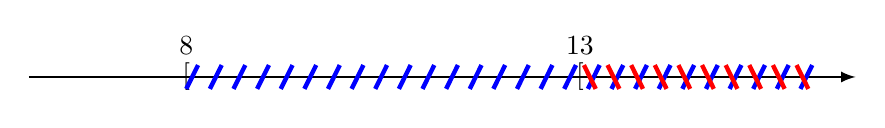
\begin{tikzpicture}[thick]
    \draw[-latex] (6,0) -- (16.5,0);
    \draw ( 8,0) node{[} node[above=1ex]{8};
    \draw (13,0) node{[} node[above=1ex]{13};
    \foreach \i in {8, 8.3, ..., 16} {
      \draw[blue, ultra thick] (\i,-1ex) -- ({\i+.15},1ex);
    }
    \foreach \i in {13, 13.3, ..., 16} {
      \draw[red, ultra thick] ({\i+.05},1ex) -- ({\i+.20},-1ex);
    }
  \end{tikzpicture}
\end{center}

Les solutions sont $x\in\left[ 8;13 \right[$.
\end{exercice}

\begin{exercice}[Coordonnées --- 3 points]
On considère la figure suivante, où $BCGH$ est un rectangle, et $EFCD$ est un carré. Répondre aux questions suivantes par lecture graphique.

\begin{multicols}{2}

\begin{center}
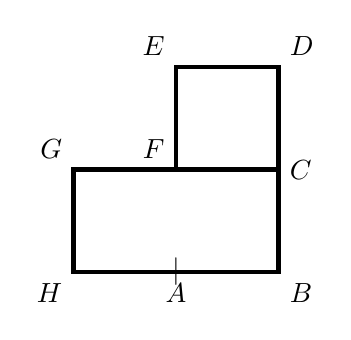
\begin{tikzpicture}[scale=1.3,ultra thick]
  \coordinate (A) at (1,0);
  \coordinate (B) at (2,0);
  \coordinate (C) at (2,1);
  \coordinate (D) at (2,2);
  \coordinate (E) at (1,2);
  \coordinate (F) at (1,1);
  \coordinate (G) at (0,1);
  \coordinate (H) at (0,0);

  \draw (H) node[below left]{$H$}
     -- (B) node[below right]{$B$}
     -- (C) node[right]{$C$}
     -- (G) node[above left]{$G$}
     -- cycle;
  \draw (A) node{$|$} node[below]{$A$};   
  \draw (C) 
     -- (D) node[above right]{$D$}
     -- (E) node[above left]{$E$}
     -- (F) node[above left]{$F$};

\end{tikzpicture}
\end{center}


\begin{enumerate}[(a)]
  \item \emph{Dans le repère $(A, B, F)$, quels points ont pour coordonnées $(-1;0)$ et $(1; 1)$ ?} $H(-1;0)$ et $C(1;1)$.
  \item \emph{Quelles sont les coordonnées de $C$ dans le repère $(H, B, G)$ ?} $C(1;1)$.
\end{enumerate}
\end{multicols}

\end{exercice}

\begin{exercice}[Problème --- 11 points]~
\begin{enumerate}[(a)]
  \item \emph{Dans un repère orthonormé, placer les points $A(2;0)$, $B(-0,5;0)$ et $C(1;2)$.}
    \begin{center}
      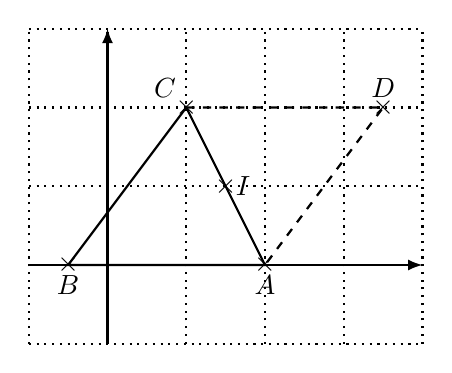
\begin{tikzpicture}[thick]
        \draw[-latex] (-1,0) -- (4,0);
        \draw[-latex] (0,-1) -- (0,3);
        \draw[dotted] (-1,-1) grid (4,3);
        \coordinate (A) at (2,0);
        \coordinate (B) at (-.5,0);
        \coordinate (C) at (1,2);
        \coordinate (D) at (3.5,2);
        \coordinate (I) at (1.5,1);
        \draw (A) node{$\times$} node[below]{$A$};
        \draw (B) node{$\times$} node[below]{$B$};
        \draw (C) node{$\times$} node[above left]{$C$};
        \draw (D) node{$\times$} node[above]{$D$};
        \draw (I) node{$\times$} node[right]{$I$};
        \draw (A) -- (B) -- (C) -- cycle;
        \draw[dashed] (C) -- (D) -- (A);
      \end{tikzpicture}
    \end{center}
    
  \item \emph{Montrer que le triangle $ABC$ est isocèle en $B$.}
    On calcule les longueurs $AB$ et $BC$.

    \begin{multicols}{2}
    \begin{align*}
      AB&=\sqrt{\left( x_B-x_A \right)^2+\left( y_B-y_A \right)^2} \\
        &=\sqrt{\left( -0,5-2  \right)^2+\left( 0  -0   \right)^2} \\
        &=\sqrt{\left( -2,5 \right)^2+0}\\
        &=\sqrt{6,25}\\
        &=2,5
    \end{align*}

    \begin{align*}
      CB&=\sqrt{\left( x_B-x_C \right)^2+\left( y_C-y_B \right)^2} \\
        &=\sqrt{\left( -1,5 \right)^2+2^2}\\
        &=\sqrt{6,25}\\
        &=2,5
    \end{align*}
  \end{multicols}
  Donc $AB=CB$, et le triangle est rectangle en $B$.
  \item \emph{Calculer les coordonnées de $I$, milieu de $\left[AC\right]$.}
    \begin{multicols}{2}
    \begin{align*}
      x_I&=\frac{x_A+x_C}{2}
         &=\frac{2+1}{2}
         &=\frac{3}{2}
    \end{align*}

    \begin{align*}
      y_I&=\frac{y_A+y_C}{2}
         &=\frac{0+2}{2}
         &=1
    \end{align*}
  \end{multicols}
  Pour vérifier que l'on a pas fait d'erreus de calcul, on peut constater sur la figure que cela correspond bien aux coordonnées de $I$.
  \item \emph{Calculer les coordonnées de $D$, symétrique de $B$ par rapport à $I$.}
    Si $D$ est le symétrique de $B$ par rapport à $I$, alors $I$ est le milieu de $BD$, donc :
    \[\systeme{
      x_I=\frac{x_B+x_D}{2}
    }{
      y_I=\frac{y_B+y_D}{2}
    }\]

    Nous connaissons les coordonnées de $I$ et $B$, donc nous obtenons :
    \[\systeme{
      \frac{3}{2}=\frac{-0,5+x_D}{2}
    }{
      1=\frac{0+y_D}{2}
    }\]
    Et ainsi, en résolvant chacune des deux équations : $x_D=3,5$, et $y_D=2$. Donc $D(3,5;2)$.
  \item \emph{Montrer que $ABCD$ est un parallélogramme.}
    Il y a plusieurs manières de montrer cela. La plus rapide est de constater que ses diagonales se coupent en leur milieu (puisque $I$ est à la fois le milieu de $BD$ et $AC$.
  \item \emph{Peut-on être plus précis sur la nature de $ABCD$ ?}
    Puisque $ABC$ est isocèle en $B$, le parallélogramme a deux côtés consécutifs de même longueur : c'est donc un losange.
\end{enumerate}
\end{exercice}

\begin{exercice}[Algorithmique -- 3 points]
  Dans un repère orthonormé, on considère le cercle $\mathcal{C}$ de centre $A(1, 0)$ et de rayon 5.
  \begin{enumerate}[(a)]
    \item \emph{Soit $B(3;5)$. Calculer la longueur $AB$. Le point $B$ appartient-il au cercle $\mathcal{C}$ ?} En utilisant la formule de la longueur d'un segment, on trouve $AB=\sqrt{\left( 3-1 \right)^2+\left( 5-0 \right)^2}$, soit $AB=\sqrt{29}$. La longueur $AB$ n'est pas 5, donc $B$ n'appartient pas au cercle $\mathcal{C}$.
    \item Compléter l'algorithme suivante, pour qu'étant données les coordonnées d'un point du plan, il détermine si oui ou non ce point fait partie du cercle $\mathcal{C}$.
  \end{enumerate}

  \begin{lstlisting}[language=naturel,frame=lines,mathescape=true]
  Lire x
  Lire y
  Si $\sqrt{\left( x-1 \right)^2+y^2}=5$
  Alors
    Afficher "Le point appartient au cercle $\mathcal{C}$"
  Sinon
    Afficher "Le point n'appartient pas au cercle $\mathcal{C}$"
  FinSi
  \end{lstlisting}

\end{exercice}

\end{document}
